\documentclass[11pt]{article}
\usepackage[textwidth=18.0cm, textheight=23.0cm, top=2.0cm]{geometry}
\usepackage{pst-all}
\usepackage{amssymb}
\usepackage{tikz}
\usepackage{underscore}\begin{document}
\pagestyle{empty}


ClassName: \underline{\textbf{Class_08.2bp-12}}
\par
BinSize: \underline{\textbf{100 × 100}}
\par
ReduceSize: \underline{\textbf{100 × 100}}
\par
TypeNum: \underline{\textbf{40}}
\par
Num: \underline{\textbf{40}}
\par
OutS: \underline{\textbf{110000}}
\par
InS: \underline{\textbf{89243}}
\par
Rate: \underline{\textbf{0.811}}
\par
UB: \underline{\textbf{11}}
\par
LB0: \underline{\textbf{11}}
\par
LB: \underline{\textbf{11}}
\par
LBWithCut: \underline{\textbf{11}}
\par
NodeCut: \underline{\textbf{0}}
\par
ExtendedNodeCnt: \underline{\textbf{1}}
\par
GenNodeCnt: \underline{\textbf{1}}
\par
PrimalNode: \underline{\textbf{0}}
\par
ColumnCount: \underline{\textbf{11}}
\par
TotalCutCount: \underline{\textbf{0}}
\par
RootCutCount: \underline{\textbf{0}}
\par
LPSolverCnt: \underline{\textbf{1}}
\par
PricingSolverCnt: \underline{\textbf{0}}
\par
BranchAndBoundNum: \underline{\textbf{1}}
\par
isOpt: \underline{\textbf{true}}
\par
TimeOnInitSolution: \underline{\textbf{0.040 s}}
\par
TimeOnPrimal: \underline{\textbf{0.000 s}}
\par
TimeOnPricing: \underline{\textbf{0.000 s}}
\par
TimeOnRmp: \underline{\textbf{0.063 s}}
\par
TotalTime: \underline{\textbf{0.165 s}}
\par
\newpage


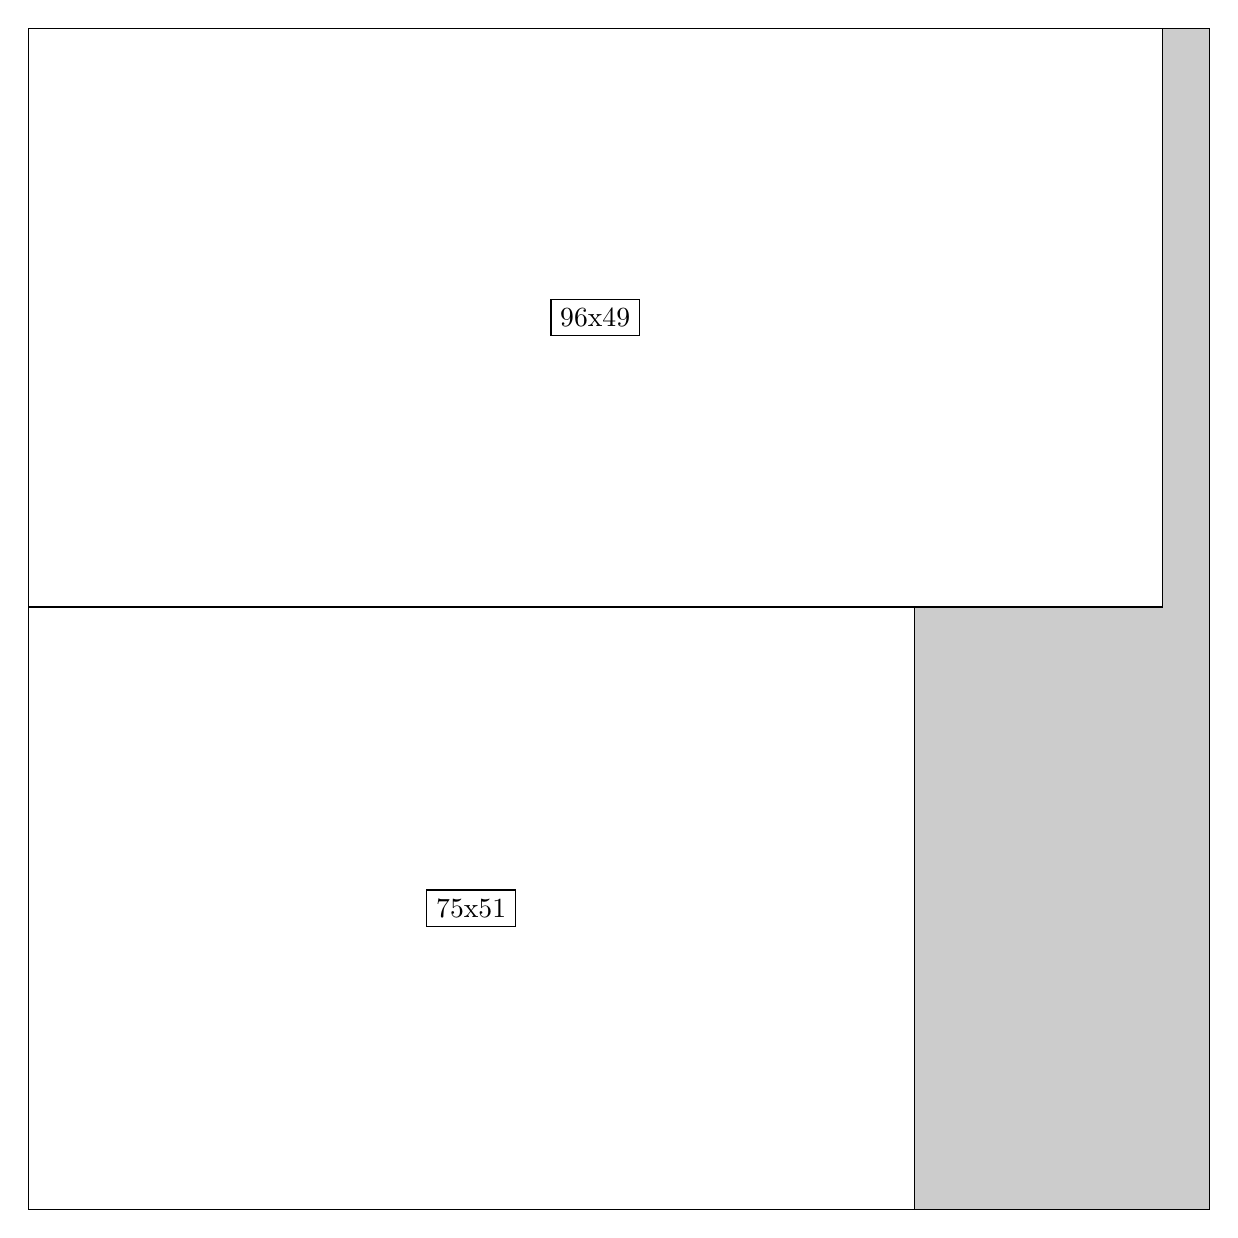
\begin{tikzpicture}[shorten >=1pt,scale=1.0,every node/.style={scale=1.0},->]
\tikzstyle{vertex}=[circle,fill=black!25,minimum size=14pt,inner sep=0pt]
\filldraw[fill=gray!40!white, draw=black] (0,0) rectangle (15.0,15.0);
\foreach \name/\x/\y/\w/\h in {96x49/0.0/7.6499999999999995/14.399999999999999/7.35,75x51/0.0/0.0/11.25/7.6499999999999995}
\filldraw[fill=white!40!white, draw=black] (\x,\y) rectangle node[draw] (\name) {\name} ++(\w,\h);
\end{tikzpicture}


w =96 , h =49 , x =0 , y =51 , v =4704
\par
w =75 , h =51 , x =0 , y =0 , v =3825
\par
\newpage


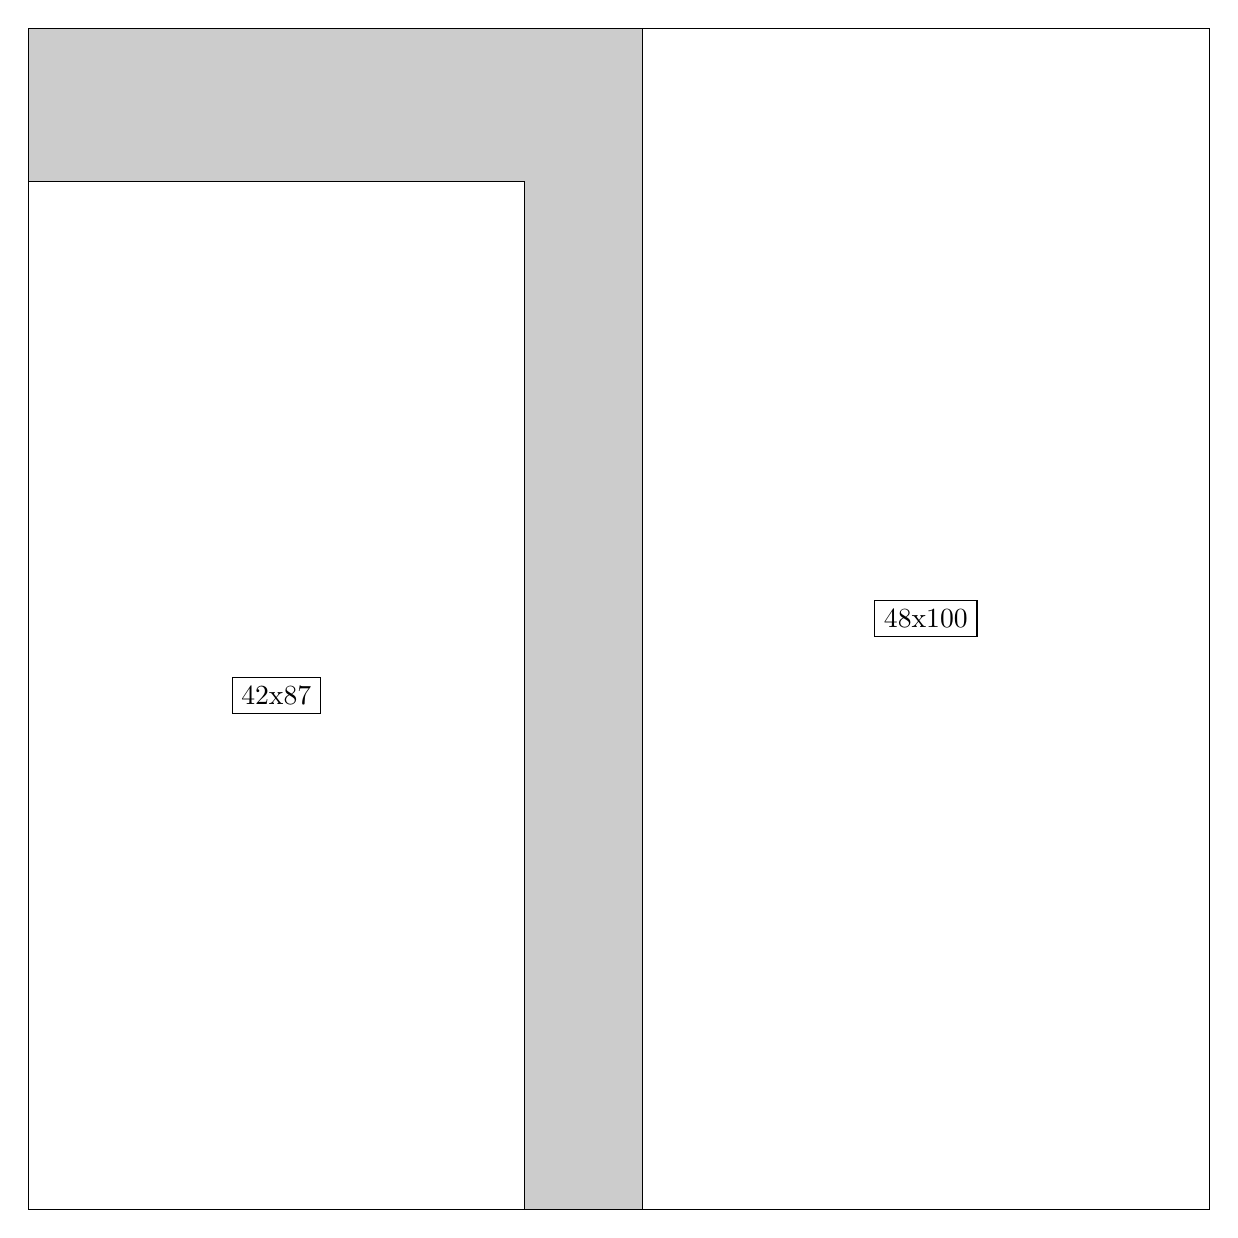
\begin{tikzpicture}[shorten >=1pt,scale=1.0,every node/.style={scale=1.0},->]
\tikzstyle{vertex}=[circle,fill=black!25,minimum size=14pt,inner sep=0pt]
\filldraw[fill=gray!40!white, draw=black] (0,0) rectangle (15.0,15.0);
\foreach \name/\x/\y/\w/\h in {48x100/7.8/0.0/7.199999999999999/15.0,42x87/0.0/0.0/6.3/13.049999999999999}
\filldraw[fill=white!40!white, draw=black] (\x,\y) rectangle node[draw] (\name) {\name} ++(\w,\h);
\end{tikzpicture}


w =48 , h =100 , x =52 , y =0 , v =4800
\par
w =42 , h =87 , x =0 , y =0 , v =3654
\par
\newpage


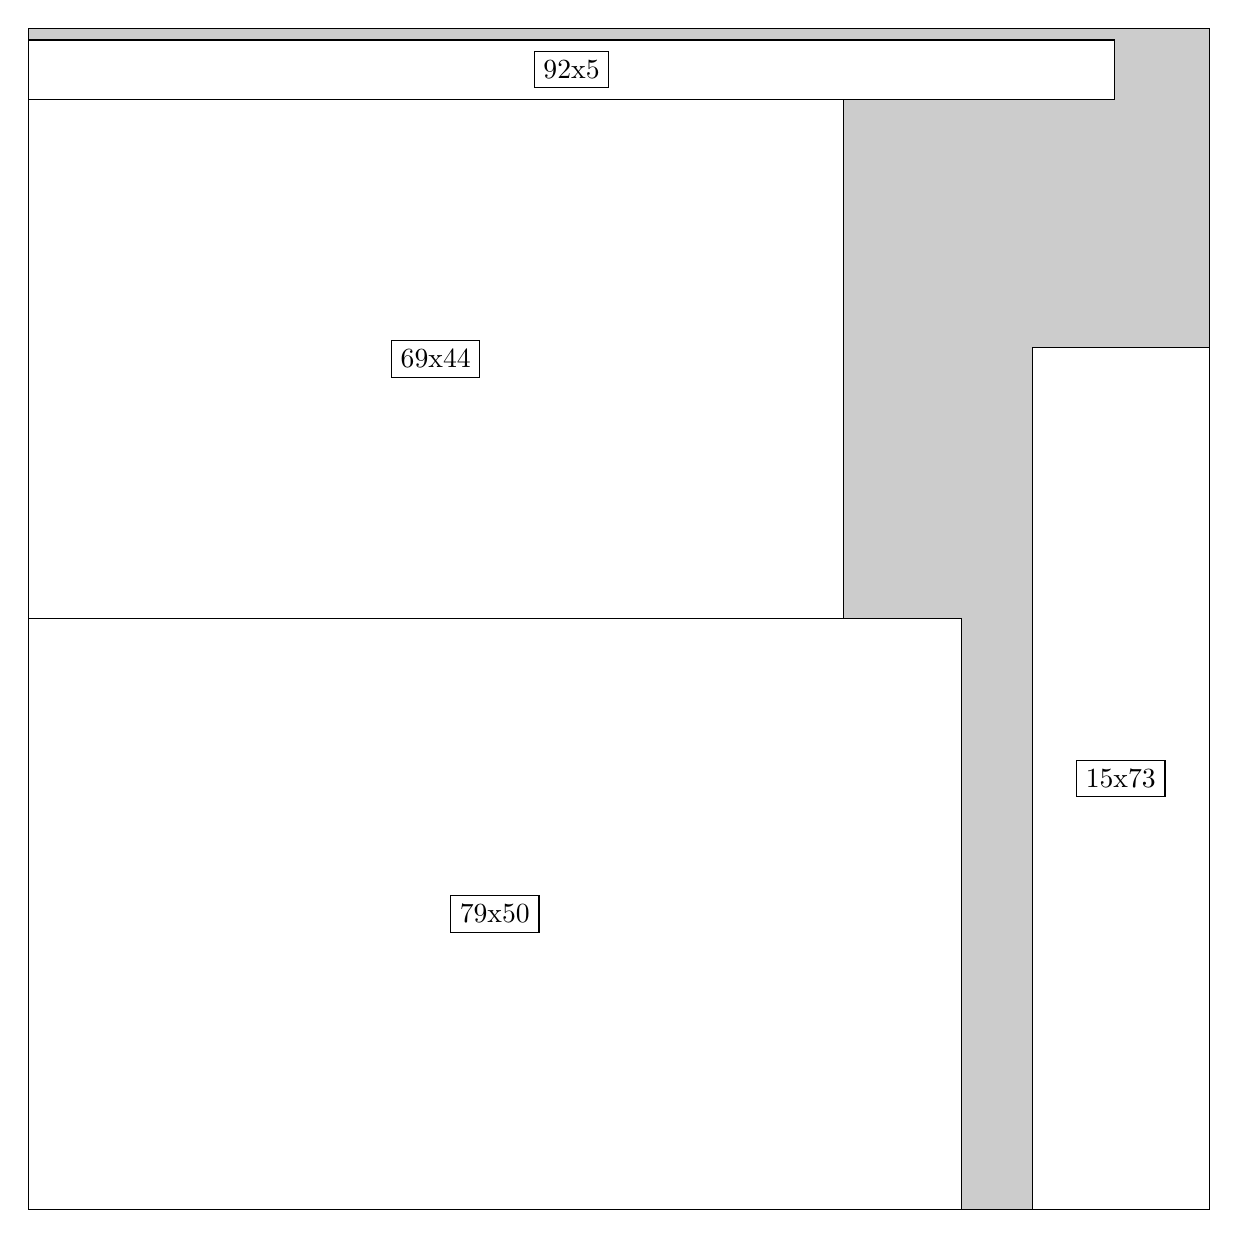
\begin{tikzpicture}[shorten >=1pt,scale=1.0,every node/.style={scale=1.0},->]
\tikzstyle{vertex}=[circle,fill=black!25,minimum size=14pt,inner sep=0pt]
\filldraw[fill=gray!40!white, draw=black] (0,0) rectangle (15.0,15.0);
\foreach \name/\x/\y/\w/\h in {79x50/0.0/0.0/11.85/7.5,69x44/0.0/7.5/10.35/6.6,15x73/12.75/0.0/2.25/10.95,92x5/0.0/14.1/13.799999999999999/0.75}
\filldraw[fill=white!40!white, draw=black] (\x,\y) rectangle node[draw] (\name) {\name} ++(\w,\h);
\end{tikzpicture}


w =79 , h =50 , x =0 , y =0 , v =3950
\par
w =69 , h =44 , x =0 , y =50 , v =3036
\par
w =15 , h =73 , x =85 , y =0 , v =1095
\par
w =92 , h =5 , x =0 , y =94 , v =460
\par
\newpage


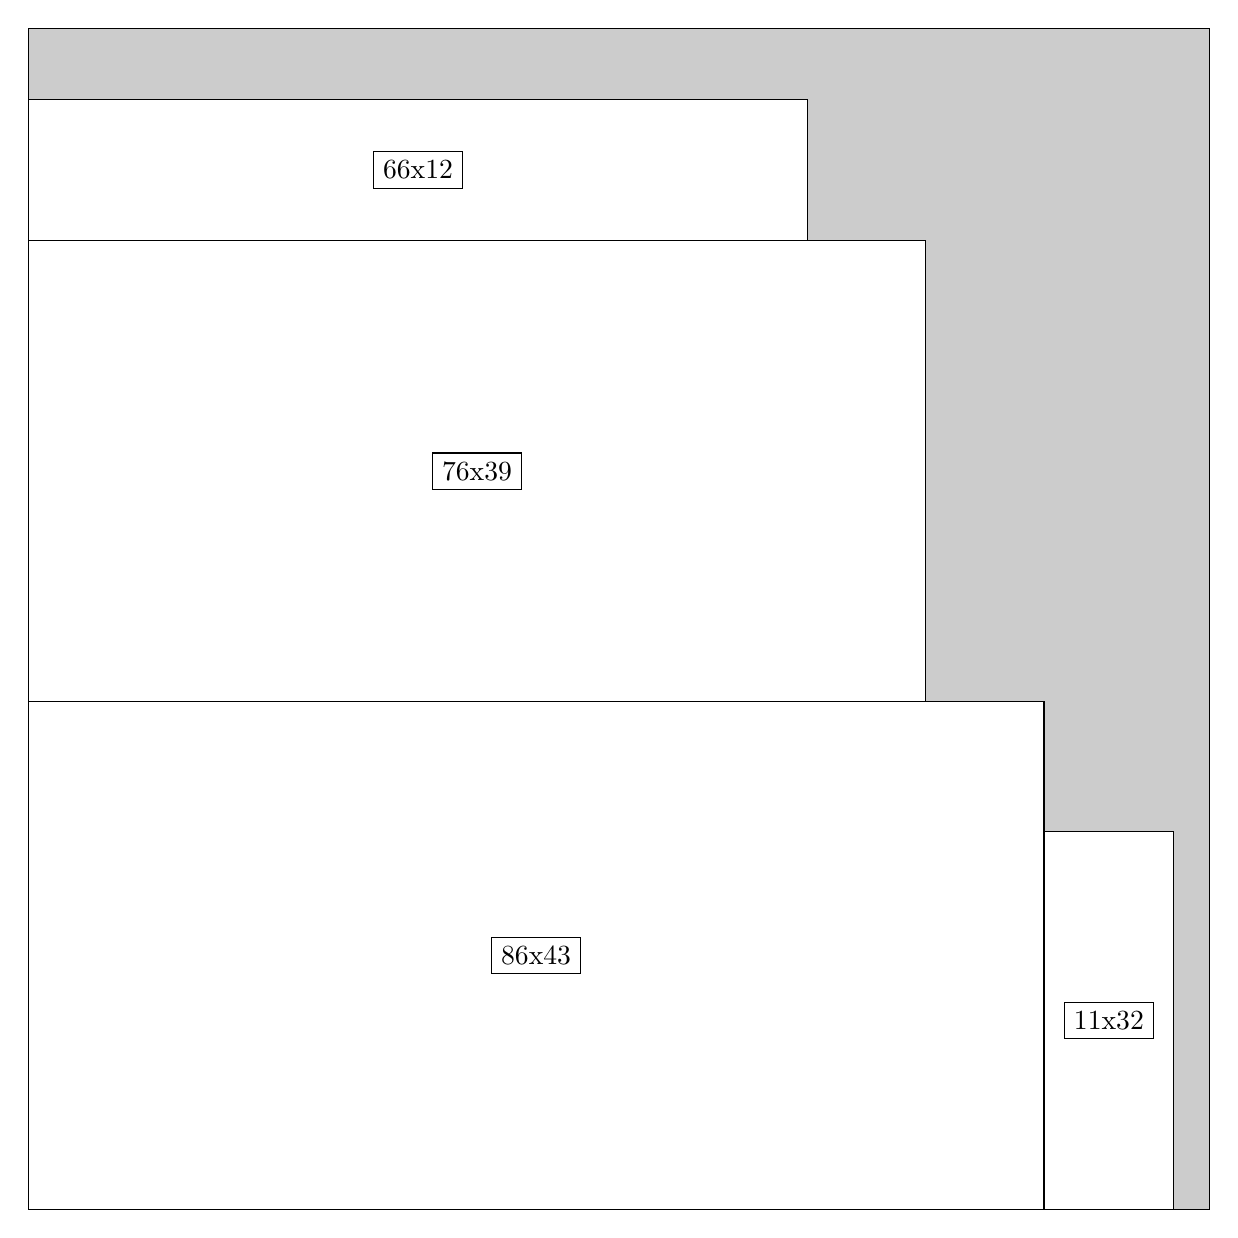
\begin{tikzpicture}[shorten >=1pt,scale=1.0,every node/.style={scale=1.0},->]
\tikzstyle{vertex}=[circle,fill=black!25,minimum size=14pt,inner sep=0pt]
\filldraw[fill=gray!40!white, draw=black] (0,0) rectangle (15.0,15.0);
\foreach \name/\x/\y/\w/\h in {86x43/0.0/0.0/12.9/6.45,76x39/0.0/6.45/11.4/5.85,66x12/0.0/12.299999999999999/9.9/1.7999999999999998,11x32/12.9/0.0/1.65/4.8}
\filldraw[fill=white!40!white, draw=black] (\x,\y) rectangle node[draw] (\name) {\name} ++(\w,\h);
\end{tikzpicture}


w =86 , h =43 , x =0 , y =0 , v =3698
\par
w =76 , h =39 , x =0 , y =43 , v =2964
\par
w =66 , h =12 , x =0 , y =82 , v =792
\par
w =11 , h =32 , x =86 , y =0 , v =352
\par
\newpage


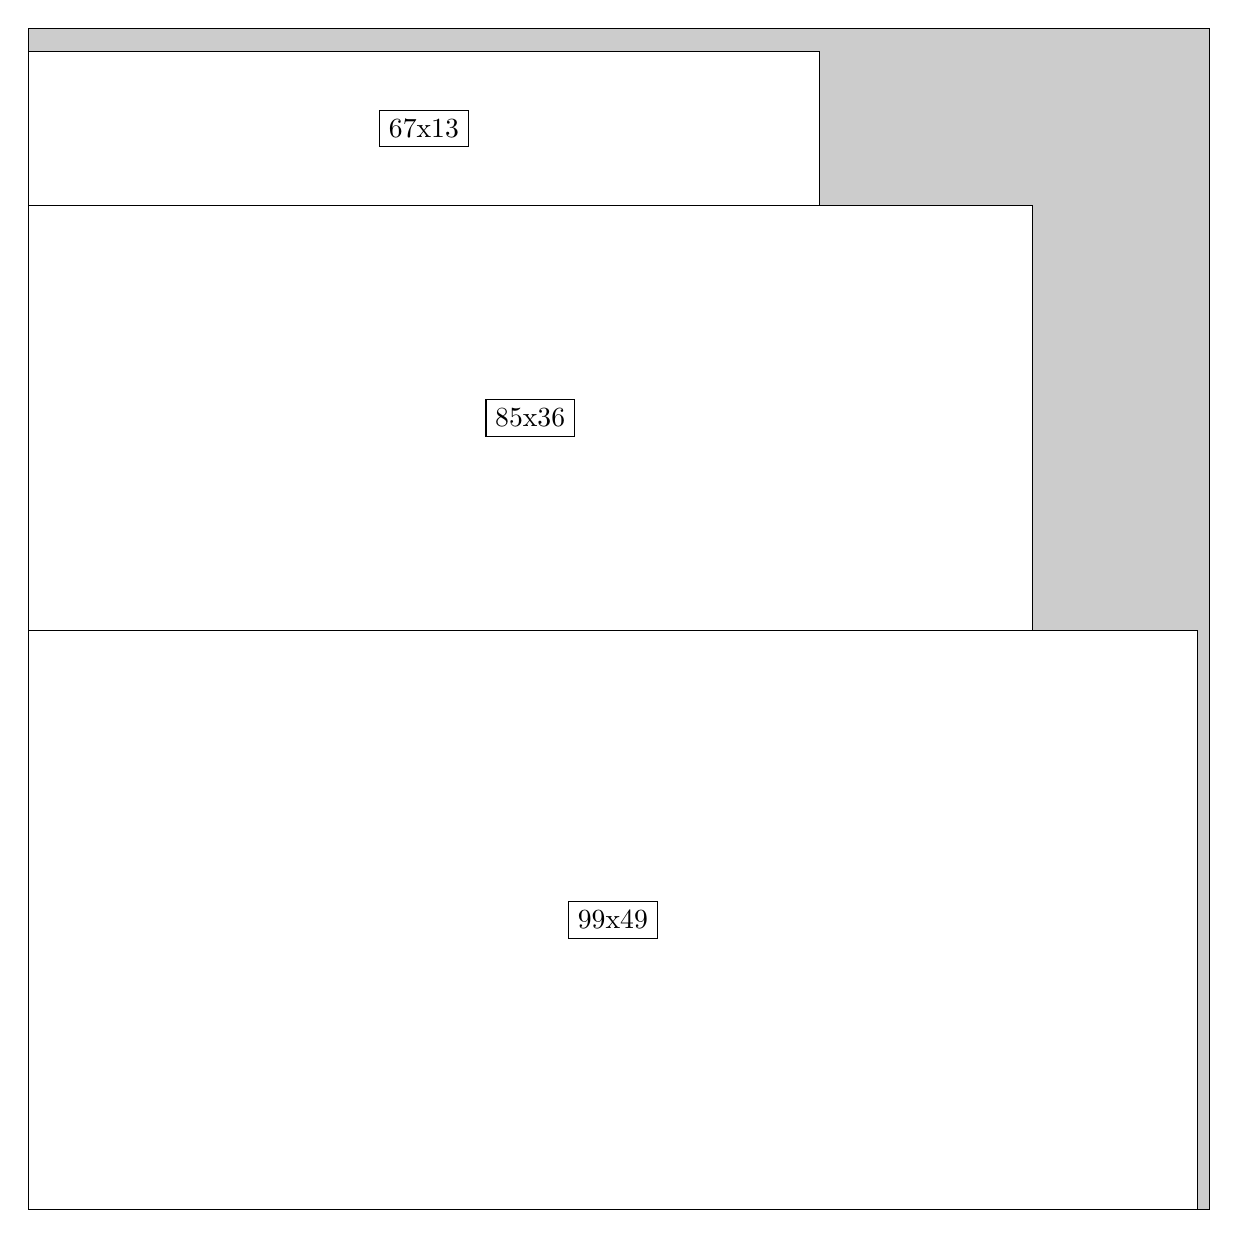
\begin{tikzpicture}[shorten >=1pt,scale=1.0,every node/.style={scale=1.0},->]
\tikzstyle{vertex}=[circle,fill=black!25,minimum size=14pt,inner sep=0pt]
\filldraw[fill=gray!40!white, draw=black] (0,0) rectangle (15.0,15.0);
\foreach \name/\x/\y/\w/\h in {99x49/0.0/0.0/14.85/7.35,85x36/0.0/7.35/12.75/5.3999999999999995,67x13/0.0/12.75/10.049999999999999/1.95}
\filldraw[fill=white!40!white, draw=black] (\x,\y) rectangle node[draw] (\name) {\name} ++(\w,\h);
\end{tikzpicture}


w =99 , h =49 , x =0 , y =0 , v =4851
\par
w =85 , h =36 , x =0 , y =49 , v =3060
\par
w =67 , h =13 , x =0 , y =85 , v =871
\par
\newpage


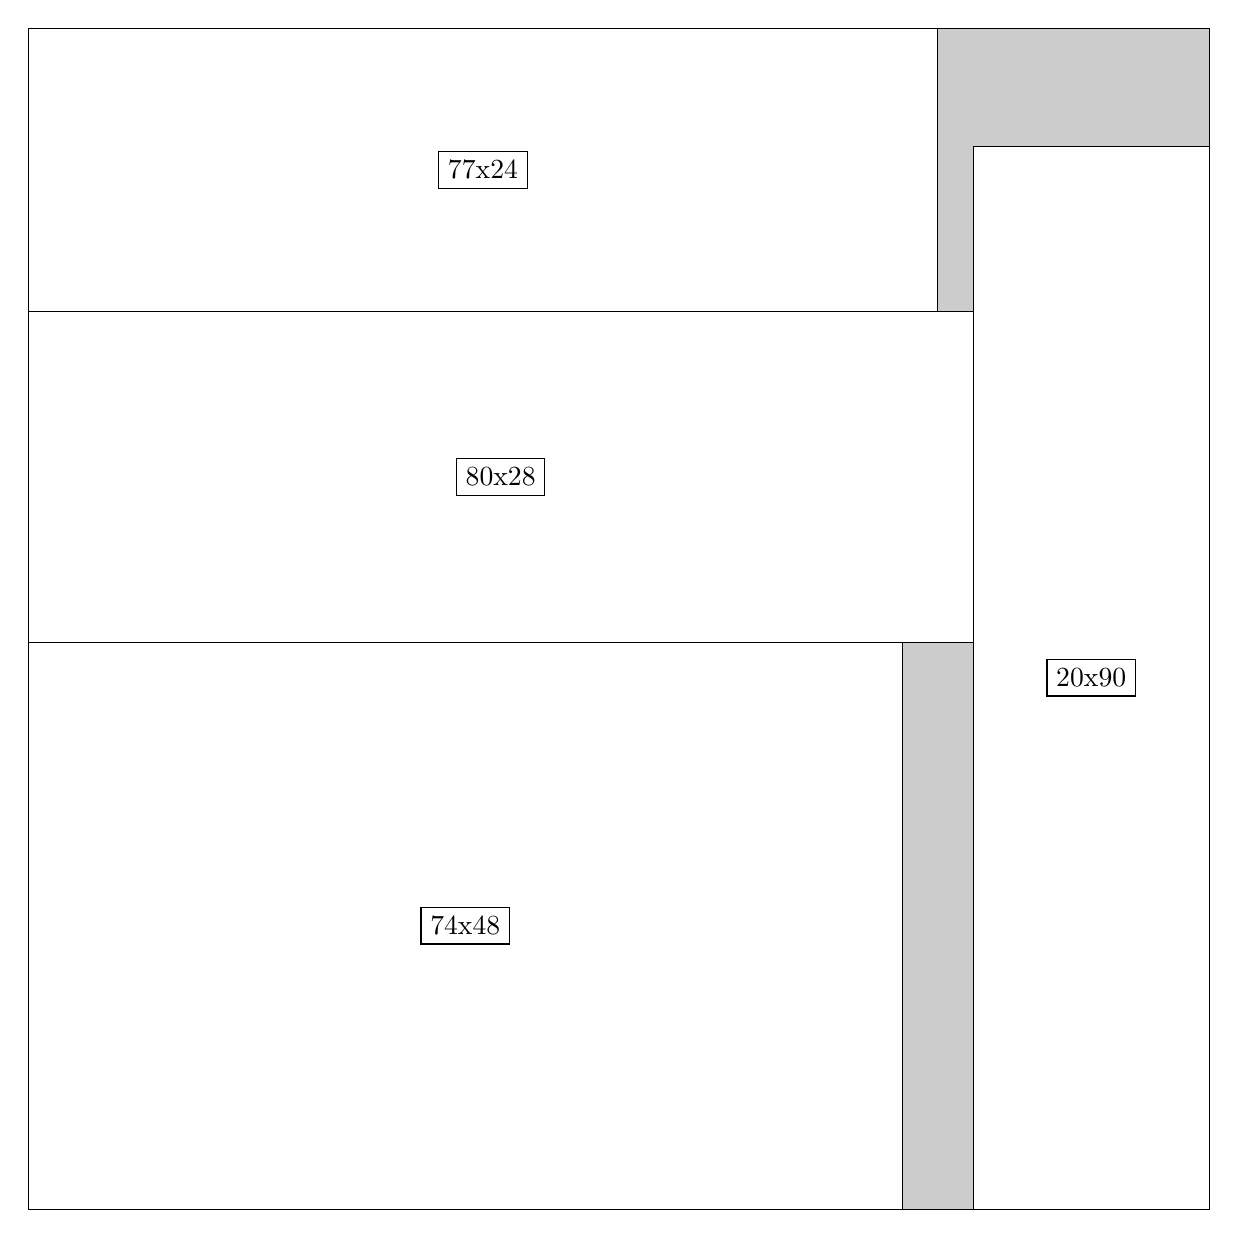
\begin{tikzpicture}[shorten >=1pt,scale=1.0,every node/.style={scale=1.0},->]
\tikzstyle{vertex}=[circle,fill=black!25,minimum size=14pt,inner sep=0pt]
\filldraw[fill=gray!40!white, draw=black] (0,0) rectangle (15.0,15.0);
\foreach \name/\x/\y/\w/\h in {74x48/0.0/0.0/11.1/7.199999999999999,80x28/0.0/7.199999999999999/12.0/4.2,77x24/0.0/11.4/11.549999999999999/3.5999999999999996,20x90/12.0/0.0/3.0/13.5}
\filldraw[fill=white!40!white, draw=black] (\x,\y) rectangle node[draw] (\name) {\name} ++(\w,\h);
\end{tikzpicture}


w =74 , h =48 , x =0 , y =0 , v =3552
\par
w =80 , h =28 , x =0 , y =48 , v =2240
\par
w =77 , h =24 , x =0 , y =76 , v =1848
\par
w =20 , h =90 , x =80 , y =0 , v =1800
\par
\newpage


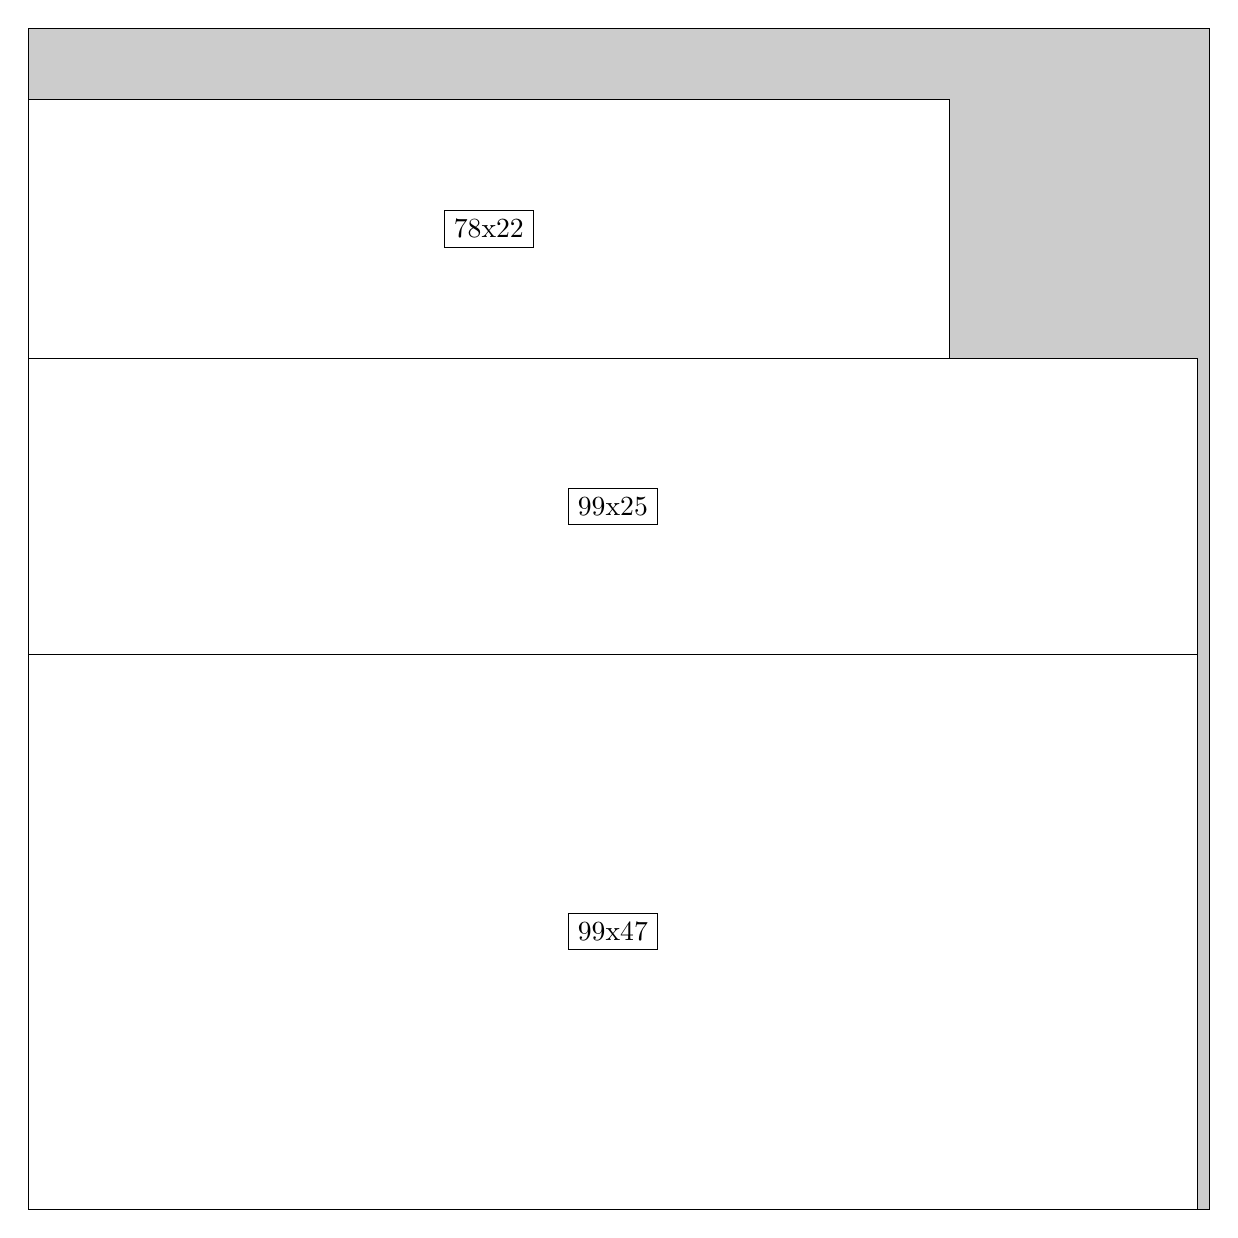
\begin{tikzpicture}[shorten >=1pt,scale=1.0,every node/.style={scale=1.0},->]
\tikzstyle{vertex}=[circle,fill=black!25,minimum size=14pt,inner sep=0pt]
\filldraw[fill=gray!40!white, draw=black] (0,0) rectangle (15.0,15.0);
\foreach \name/\x/\y/\w/\h in {99x47/0.0/0.0/14.85/7.05,99x25/0.0/7.05/14.85/3.75,78x22/0.0/10.799999999999999/11.7/3.3}
\filldraw[fill=white!40!white, draw=black] (\x,\y) rectangle node[draw] (\name) {\name} ++(\w,\h);
\end{tikzpicture}


w =99 , h =47 , x =0 , y =0 , v =4653
\par
w =99 , h =25 , x =0 , y =47 , v =2475
\par
w =78 , h =22 , x =0 , y =72 , v =1716
\par
\newpage


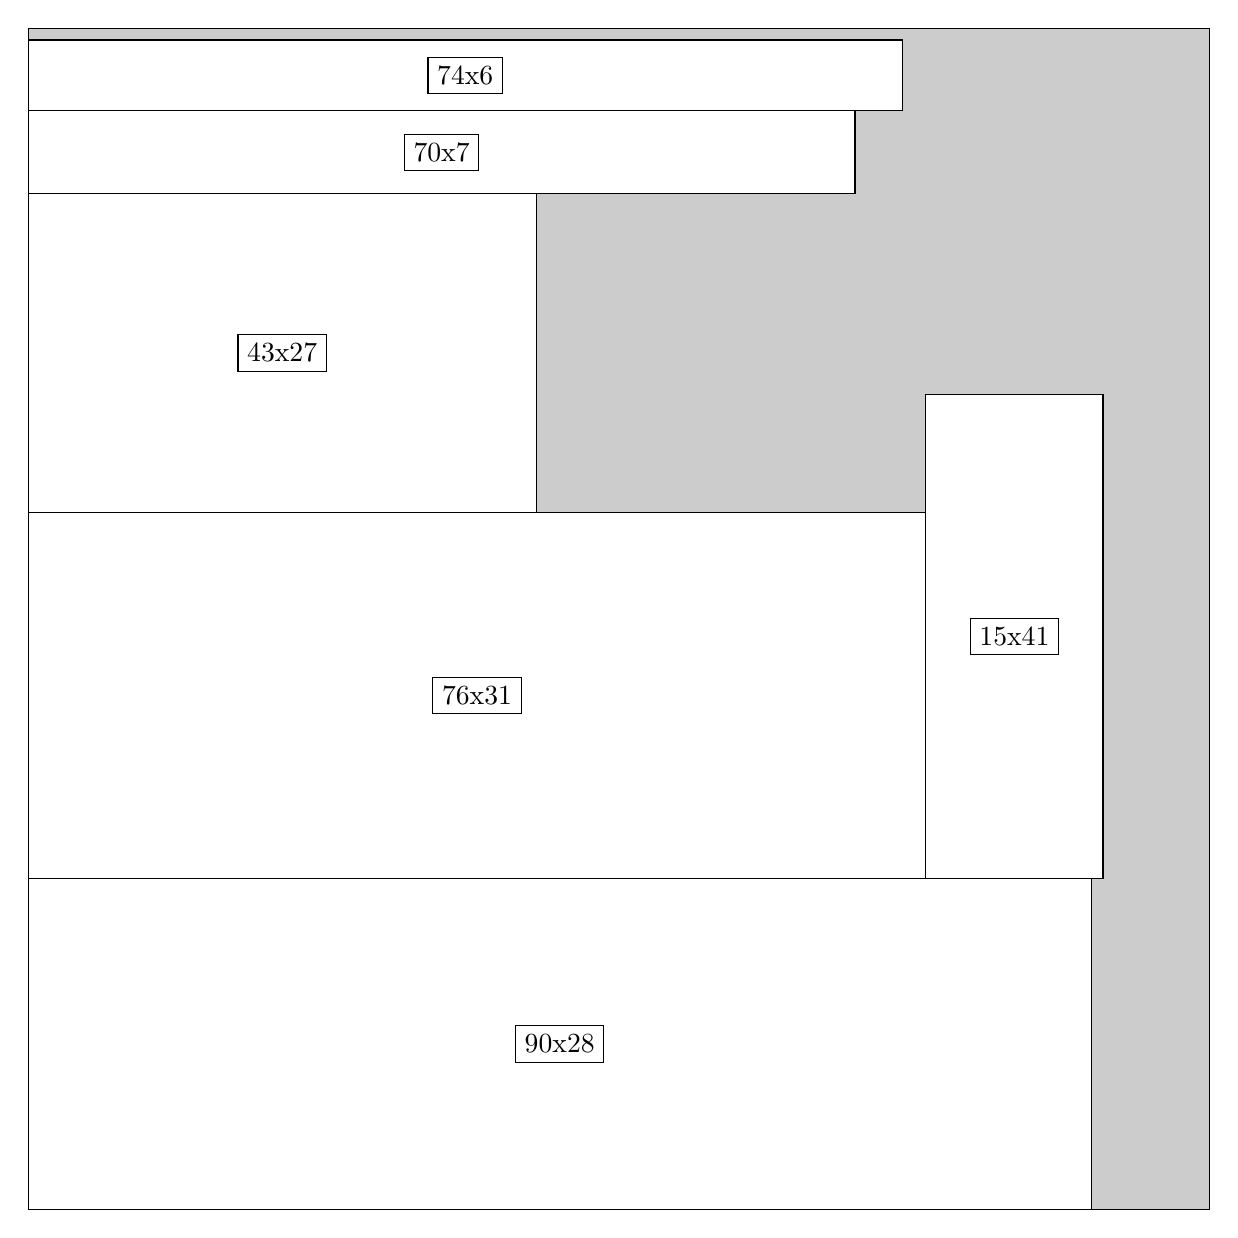
\begin{tikzpicture}[shorten >=1pt,scale=1.0,every node/.style={scale=1.0},->]
\tikzstyle{vertex}=[circle,fill=black!25,minimum size=14pt,inner sep=0pt]
\filldraw[fill=gray!40!white, draw=black] (0,0) rectangle (15.0,15.0);
\foreach \name/\x/\y/\w/\h in {90x28/0.0/0.0/13.5/4.2,76x31/0.0/4.2/11.4/4.6499999999999995,43x27/0.0/8.85/6.45/4.05,70x7/0.0/12.9/10.5/1.05,15x41/11.4/4.2/2.25/6.1499999999999995,74x6/0.0/13.95/11.1/0.8999999999999999}
\filldraw[fill=white!40!white, draw=black] (\x,\y) rectangle node[draw] (\name) {\name} ++(\w,\h);
\end{tikzpicture}


w =90 , h =28 , x =0 , y =0 , v =2520
\par
w =76 , h =31 , x =0 , y =28 , v =2356
\par
w =43 , h =27 , x =0 , y =59 , v =1161
\par
w =70 , h =7 , x =0 , y =86 , v =490
\par
w =15 , h =41 , x =76 , y =28 , v =615
\par
w =74 , h =6 , x =0 , y =93 , v =444
\par
\newpage


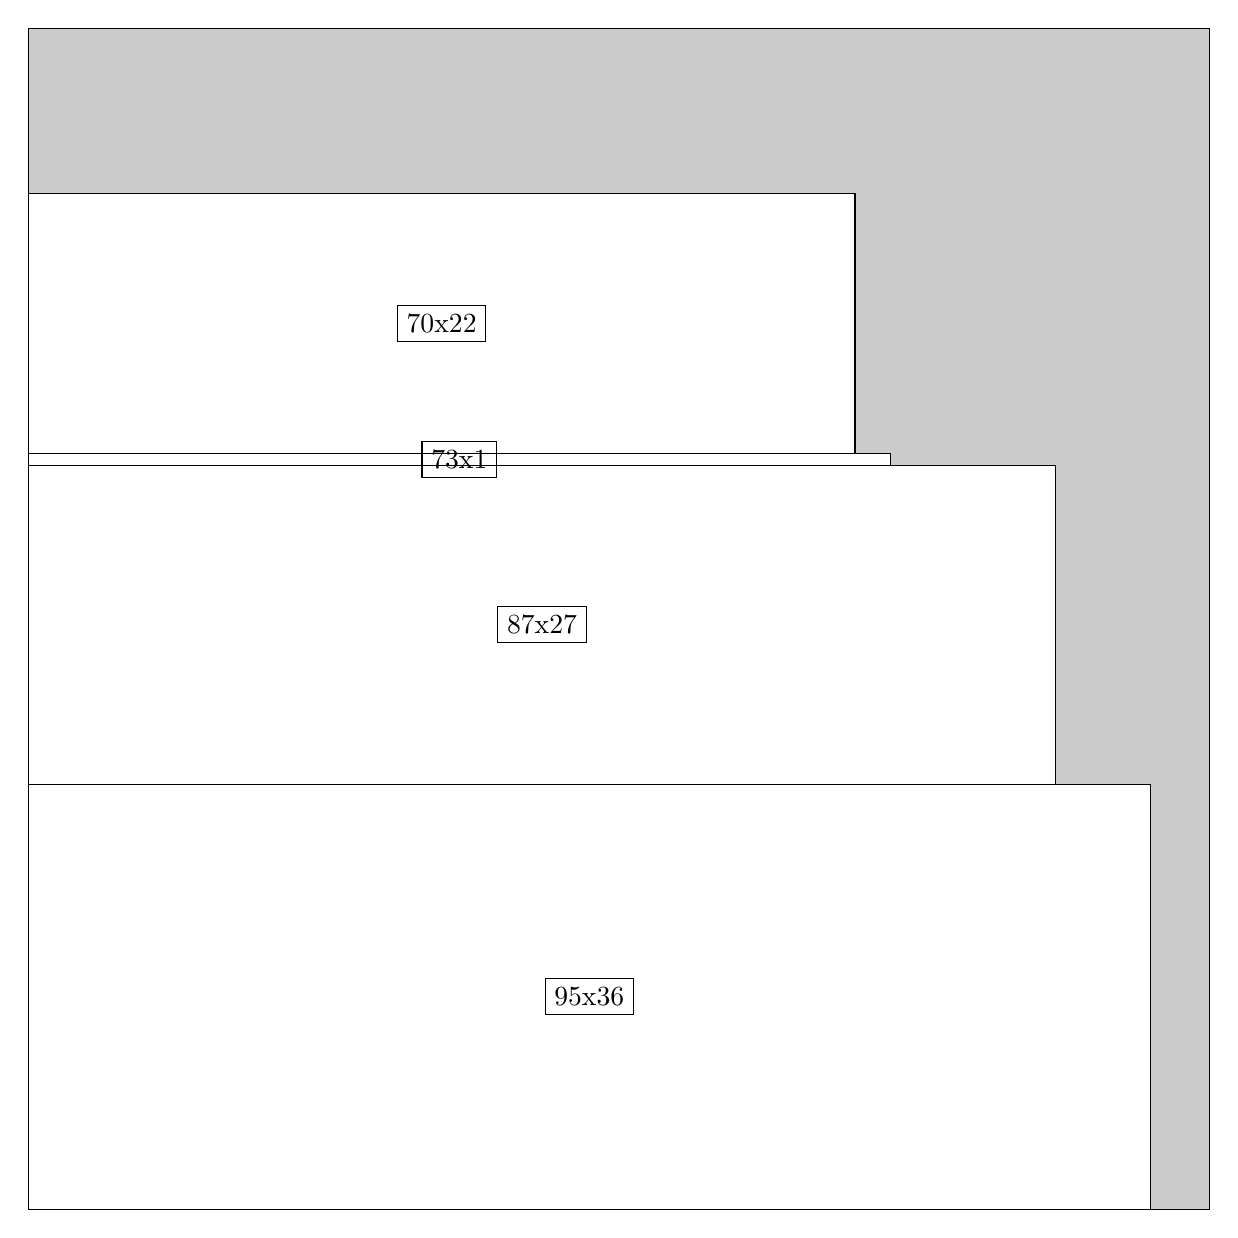
\begin{tikzpicture}[shorten >=1pt,scale=1.0,every node/.style={scale=1.0},->]
\tikzstyle{vertex}=[circle,fill=black!25,minimum size=14pt,inner sep=0pt]
\filldraw[fill=gray!40!white, draw=black] (0,0) rectangle (15.0,15.0);
\foreach \name/\x/\y/\w/\h in {95x36/0.0/0.0/14.25/5.3999999999999995,87x27/0.0/5.3999999999999995/13.049999999999999/4.05,70x22/0.0/9.6/10.5/3.3,73x1/0.0/9.45/10.95/0.15}
\filldraw[fill=white!40!white, draw=black] (\x,\y) rectangle node[draw] (\name) {\name} ++(\w,\h);
\end{tikzpicture}


w =95 , h =36 , x =0 , y =0 , v =3420
\par
w =87 , h =27 , x =0 , y =36 , v =2349
\par
w =70 , h =22 , x =0 , y =64 , v =1540
\par
w =73 , h =1 , x =0 , y =63 , v =73
\par
\newpage


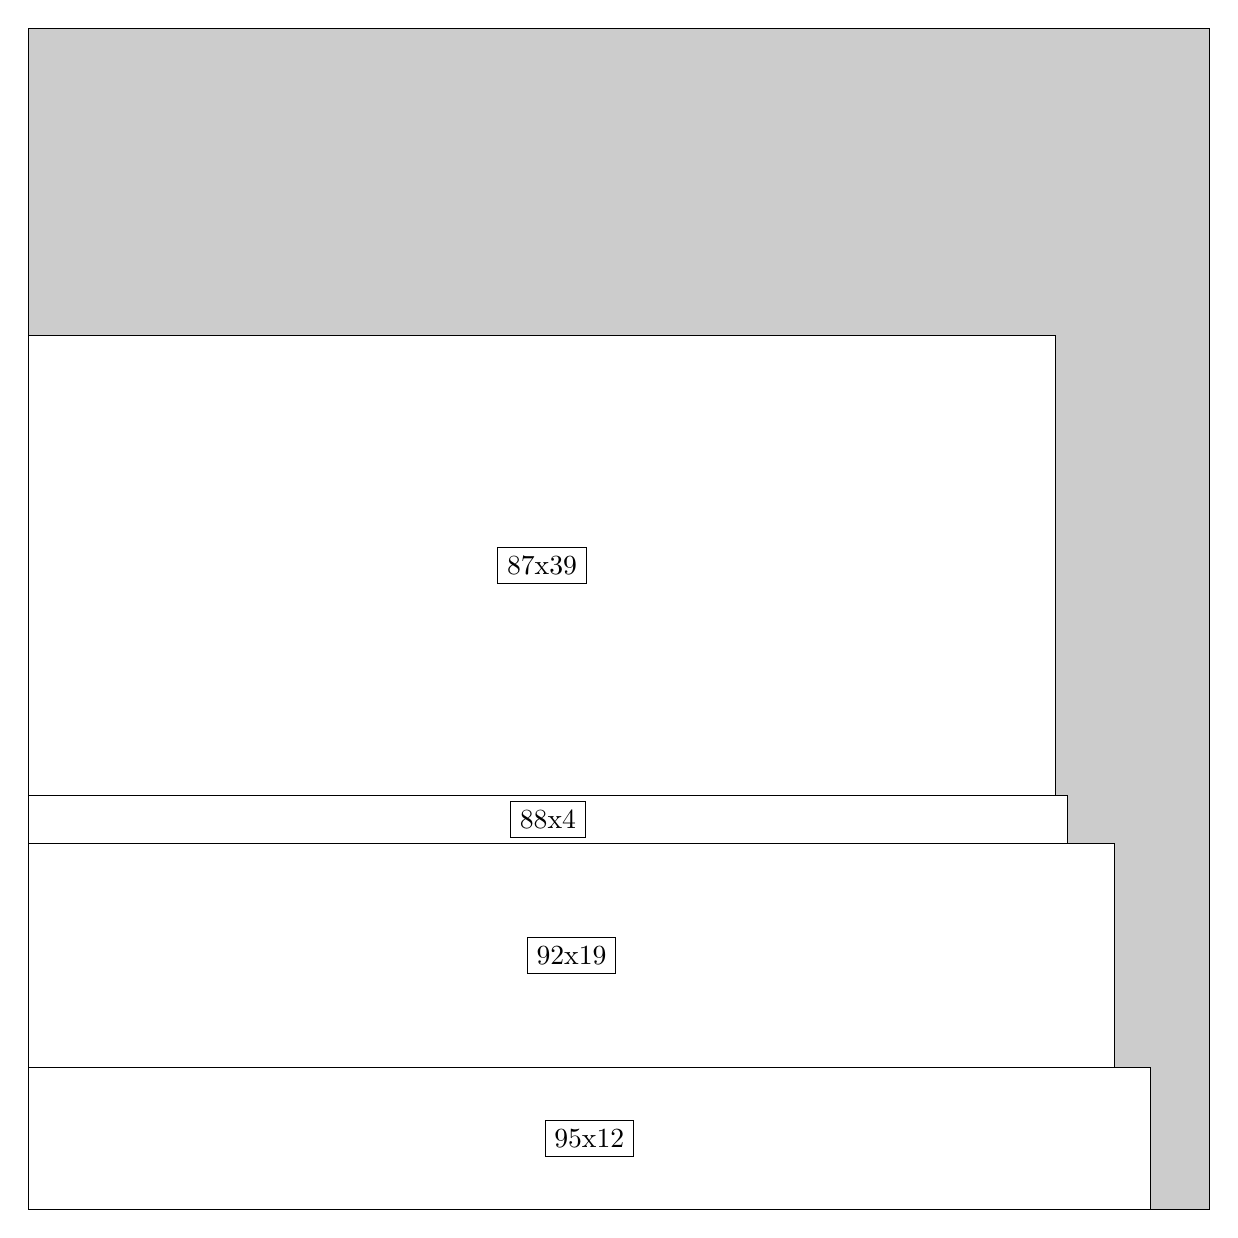
\begin{tikzpicture}[shorten >=1pt,scale=1.0,every node/.style={scale=1.0},->]
\tikzstyle{vertex}=[circle,fill=black!25,minimum size=14pt,inner sep=0pt]
\filldraw[fill=gray!40!white, draw=black] (0,0) rectangle (15.0,15.0);
\foreach \name/\x/\y/\w/\h in {87x39/0.0/5.25/13.049999999999999/5.85,92x19/0.0/1.7999999999999998/13.799999999999999/2.85,95x12/0.0/0.0/14.25/1.7999999999999998,88x4/0.0/4.6499999999999995/13.2/0.6}
\filldraw[fill=white!40!white, draw=black] (\x,\y) rectangle node[draw] (\name) {\name} ++(\w,\h);
\end{tikzpicture}


w =87 , h =39 , x =0 , y =35 , v =3393
\par
w =92 , h =19 , x =0 , y =12 , v =1748
\par
w =95 , h =12 , x =0 , y =0 , v =1140
\par
w =88 , h =4 , x =0 , y =31 , v =352
\par
\newpage


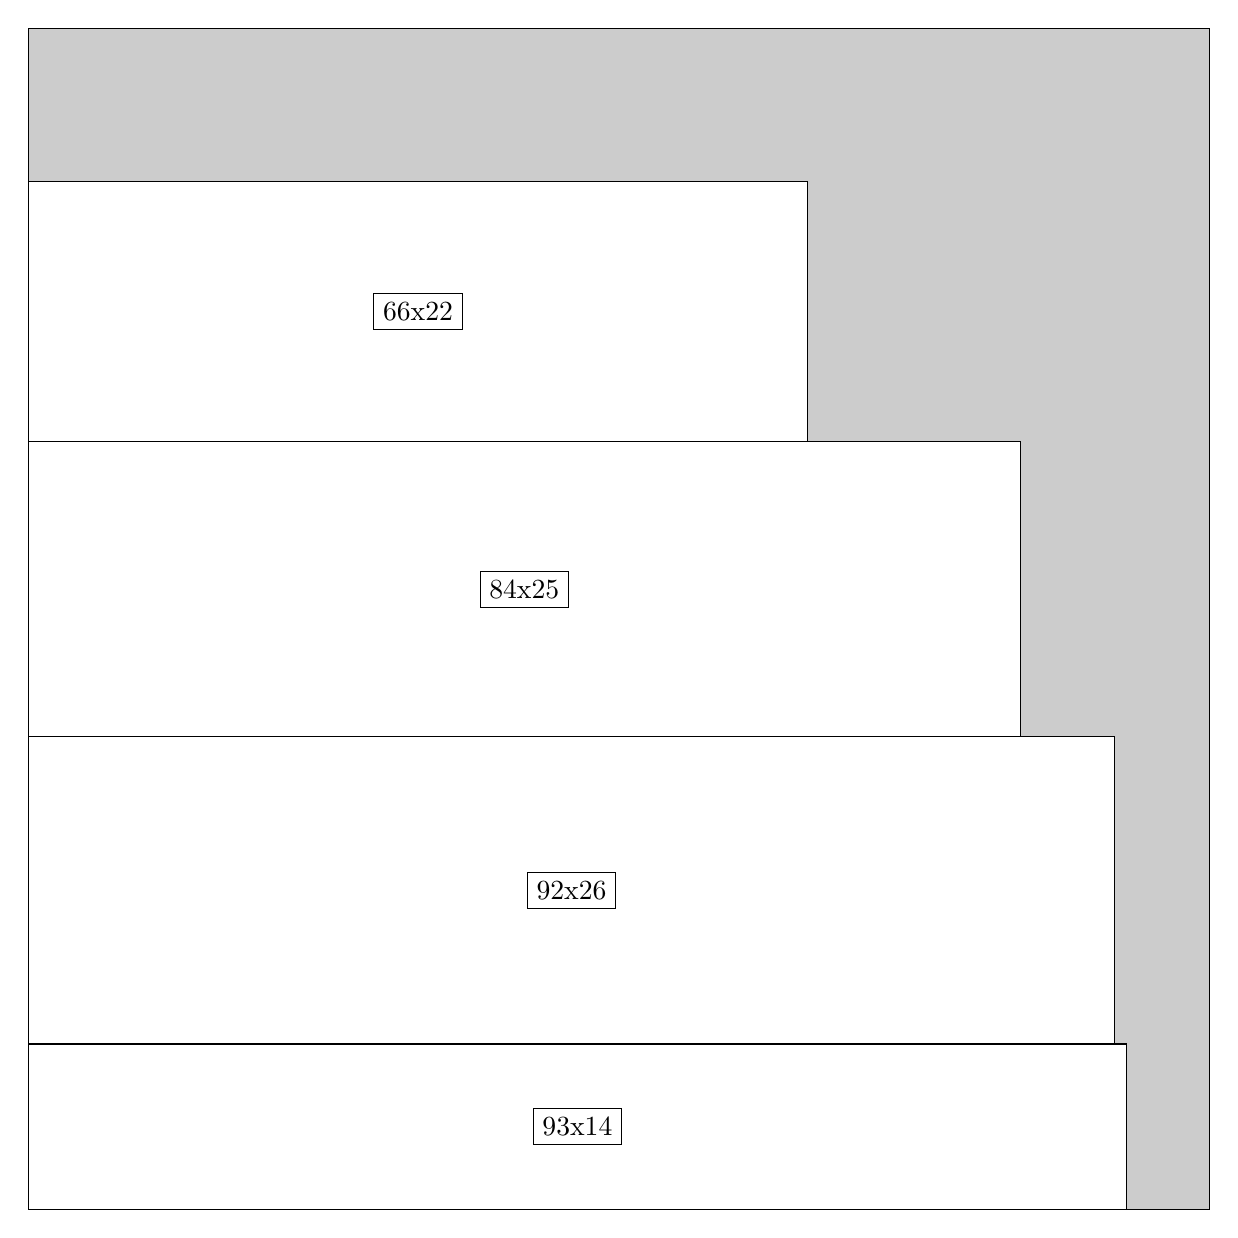
\begin{tikzpicture}[shorten >=1pt,scale=1.0,every node/.style={scale=1.0},->]
\tikzstyle{vertex}=[circle,fill=black!25,minimum size=14pt,inner sep=0pt]
\filldraw[fill=gray!40!white, draw=black] (0,0) rectangle (15.0,15.0);
\foreach \name/\x/\y/\w/\h in {92x26/0.0/2.1/13.799999999999999/3.9,84x25/0.0/6.0/12.6/3.75,66x22/0.0/9.75/9.9/3.3,93x14/0.0/0.0/13.95/2.1}
\filldraw[fill=white!40!white, draw=black] (\x,\y) rectangle node[draw] (\name) {\name} ++(\w,\h);
\end{tikzpicture}


w =92 , h =26 , x =0 , y =14 , v =2392
\par
w =84 , h =25 , x =0 , y =40 , v =2100
\par
w =66 , h =22 , x =0 , y =65 , v =1452
\par
w =93 , h =14 , x =0 , y =0 , v =1302
\par
\newpage


\end{document}